\section{Results}\label{results2d}
We first present results from FARGO simulations. The 2D disc spans
$[R_\mathrm{min}, R_\mathrm{max}] = [0.4,10]R_0$. This gives a total
disc mass $M_{d}=0.086M_*$. The mass within
$R\in[R_\mathrm{min},R_{1}]$ is $0.017M_*$, that within
$R\in[R_{1},R_{2}]$ is $0.049M_*$, and that within
$R\in[R_{2},R_\mathrm{max}]$ is $0.021M_*$. We use a resolution of
$N_R\times N_\phi = 1024\times 2048$, or about $16$ grids per $H$, and
adopt $\epsilon_g=10^{-4}hR$ for the   
self-gravity softening length\footnote{In 2D self-gravity, $\epsilon_g$ also
  approximates for the vertical disc thickness, so a more appropriate
  value would be $\epsilon_g\sim H$ \citep{muller12}. However, because
  $\epsilon_g\propto R$ is needed in FARGO, the Poisson kernel
  (Eq. \ref{2d_grav}) is no longer symmetric in $(R,R^\prime)$. We
  choose a small  
  $\epsilon_g$ in favour of angular momentum conservation, keeping in
  mind that the strength of self-gravity will be over-estimated.}.

In these simulations the disc is subject to initial perturbations in 
cylindrical radial velocity, 
\begin{align}\label{randpert}
  v_R \to v_R+ c_s\frac{\delta}{M}
  \exp{\left[-\frac{1}{2}\left(\frac{R-\overline{R}}{\Delta 
          R}\right)^2\right]}\sum_{m=1}^M\cos{m\phi},
\end{align}
where the amplitude $\delta\in[-10^{-3},10^{-3}]$ is set randomly but
independent of $\phi$, $\overline{R} = (R_{1}+R_{2})/2$
and $\Delta R = (R_{2}-R_{1})/2$. 

\subsection{Reference run}
To obtain a picture of the overall disc evolution, we describe a 
fiducial run initialised with $M=10$ in Eq. \ref{randpert}. 
Fig. \ref{fargo_modeamp} plots evolution of the maximum 
non-axisymmetric surface density amplitudes in $R\in[R_{1},R_{2}]$
for $m\in[1,10]$. Snapshots from the simulation are shown in
Fig. \ref{fargo_2d}. 
At early times $t\lesssim100P_0$ the disc 
dominated by low-amplitude high-$m$ perturbations. The $m\geq4$ modes
growth initially and saturate (or decays) after $t=40P_0$. Notice the
low $m\leq 2$ modes decay initially, but grows between $t\in[20,40]P_0$,
possibly due to non-linear interaction of the high-$m$ modes  
\citep{laughlin96,laughlin97}. However, the $m=1$ mode begins to grow
again after $t=70P_0$, and eventually dominates the annulus. 

\begin{figure}
  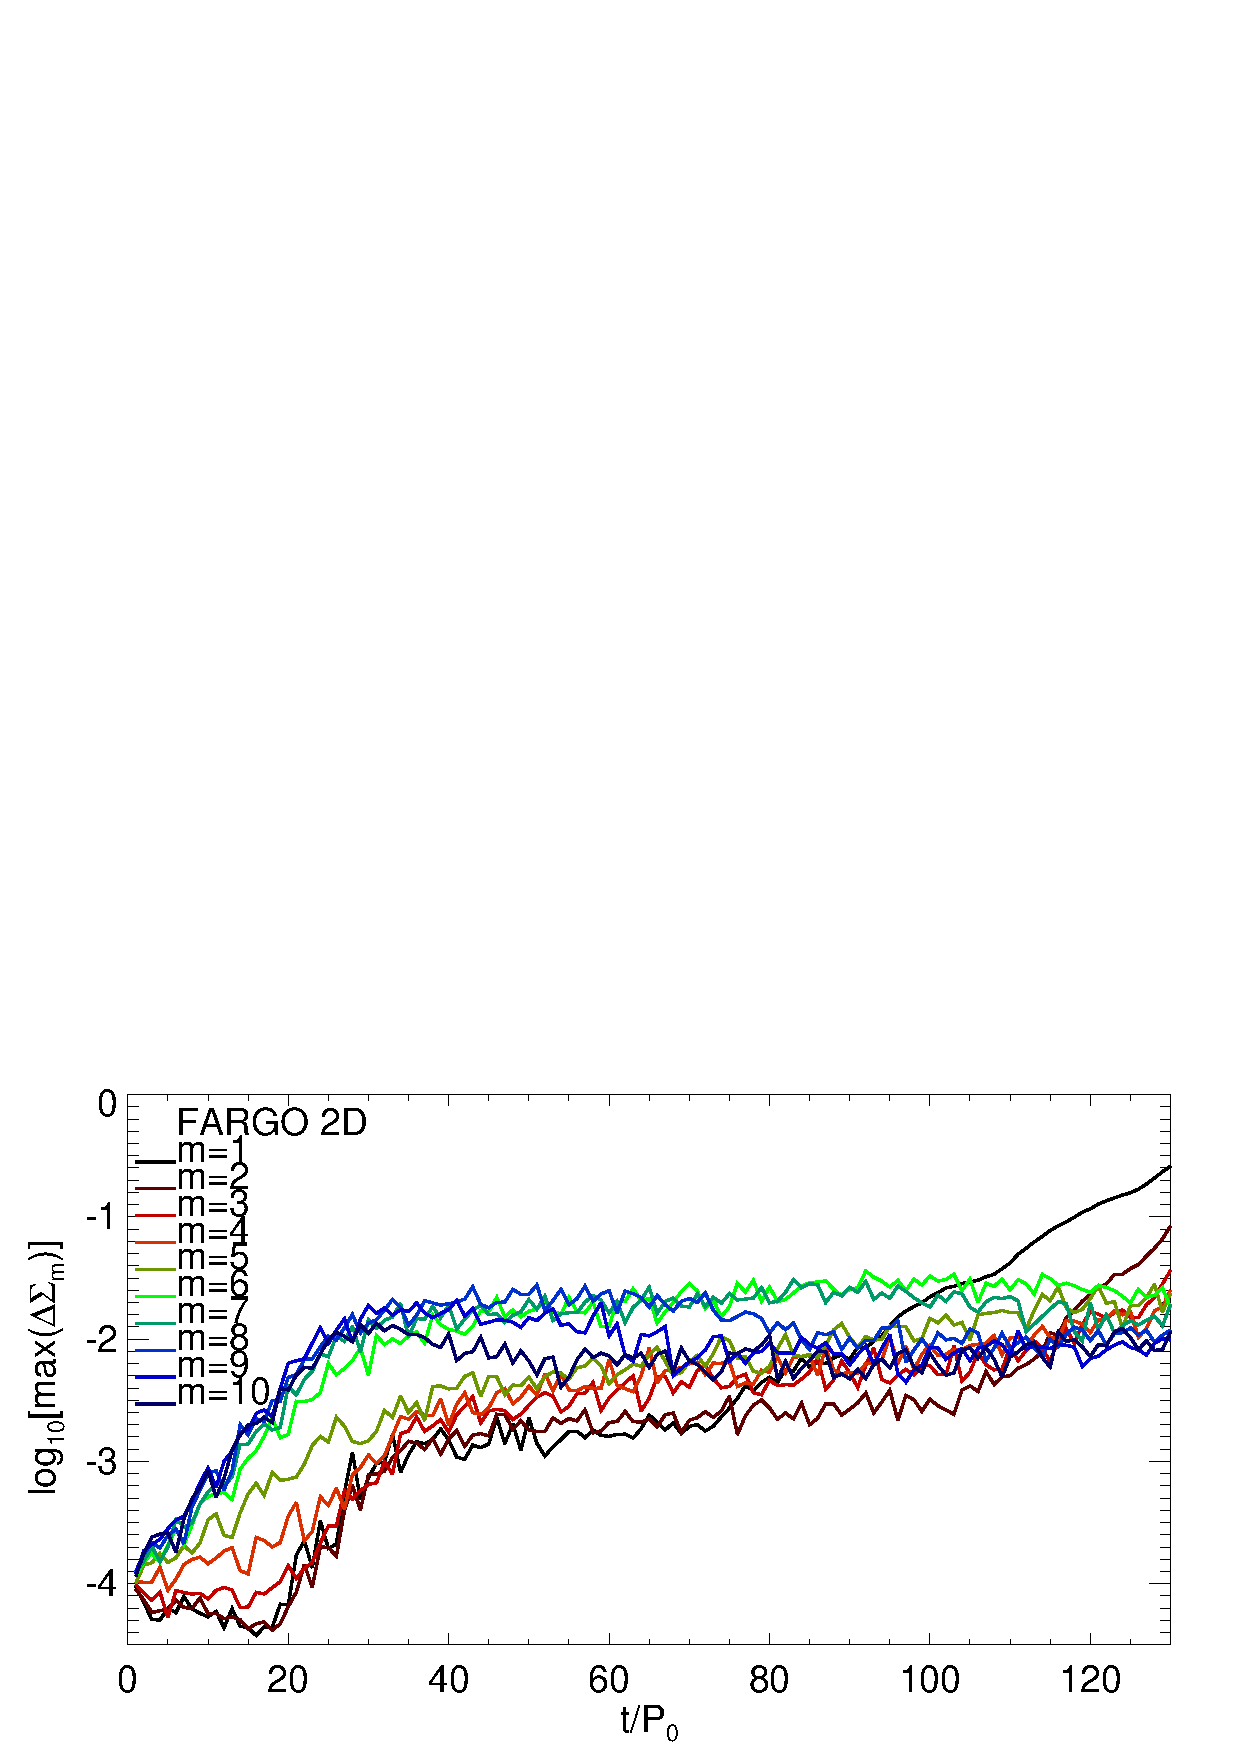
\includegraphics[width=\linewidth]{figures/nonaxi_evol_DZ_fargo}
  \caption{Evolution of non-axisymmetric surface density maxima 
    in the FARGO simulation initialised with perturbations
    with $m\in[1,10]$.\label{fargo_modeamp}} 
\end{figure}

\begin{figure}
  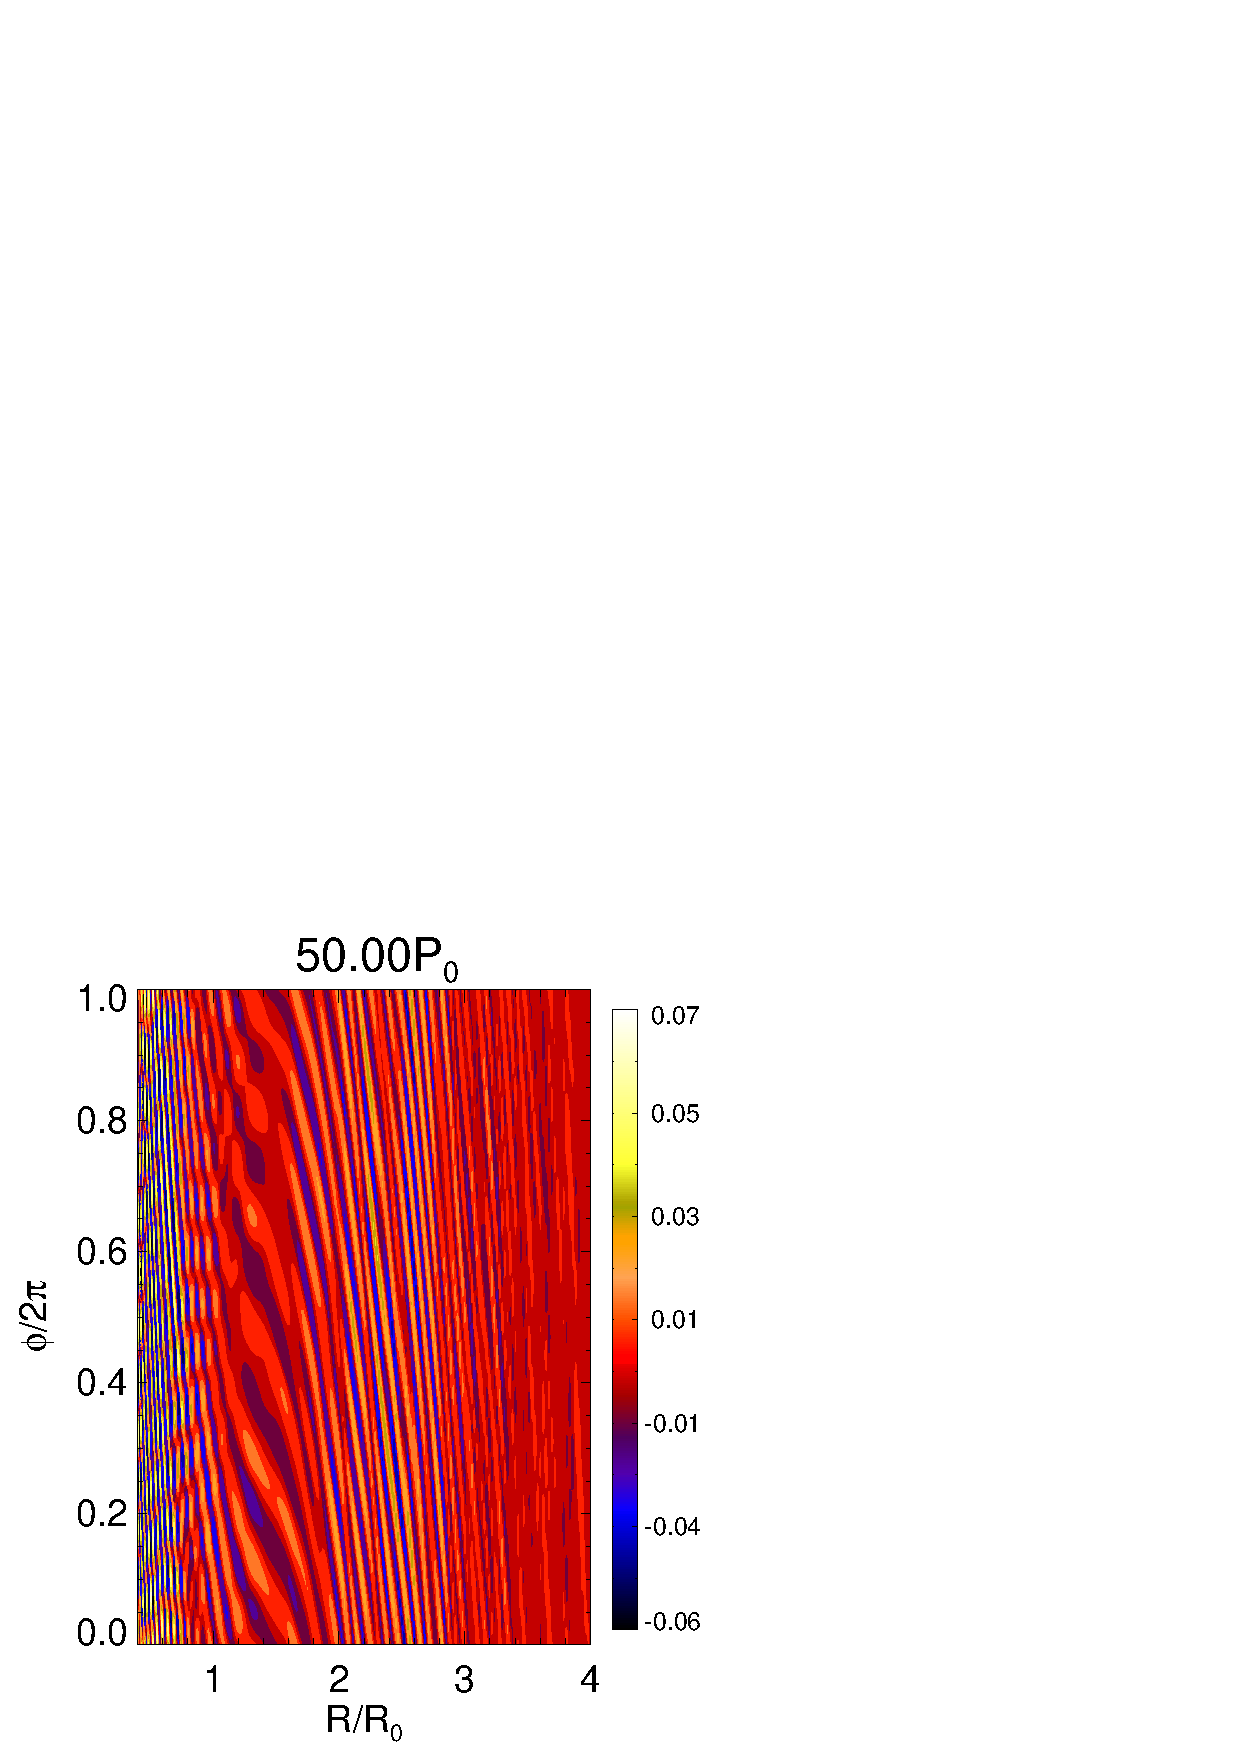
\includegraphics[scale=0.27]{figures/polarxy_dens050}\includegraphics[scale=0.27,clip=true,trim=2.26cm 
  0cm 0cm 
  0cm]{figures/polarxy_dens110}\includegraphics[scale=0.27,clip=true,trim=2.26cm
  0cm 0cm 0cm]{figures/polarxy_dens130} 
  \caption{Visualisation of the FARGO 2D simulation in
    Fig. \ref{fargo_modeamp}. The total  
    non-axisymmetric surface density
    $\Delta\Sigma$ is shown. \label{fargo_2d}} 
\end{figure}

Fig. \ref{2d_angmom} shows the evolution of disc angular momentum
components. Only the $m=0,\,1$ components are 
plotted since they are dominant. The $m=1$ structure has
an associated negative angular momentum.  
Its growth is compensated by an increase in the axisymmetric
component of angular momentum, such that $\Delta J_0 + \Delta
J_1 \sim 0$. Note that FARGO does not conserve angular momentum
exactly. However, we find the total angular momentum varies by 
$|\Delta J/J|= O(10^{-6})$, and is much smaller than the
change in the angular momenta components, $|\Delta J_{0,1}/J|>
O(10^{-5})$. Fig. \ref{2d_angmom} then suggest that angular momentum
is transferred from the one-armed spiral to the background disc.    

\begin{figure}
  % scale=0.41
  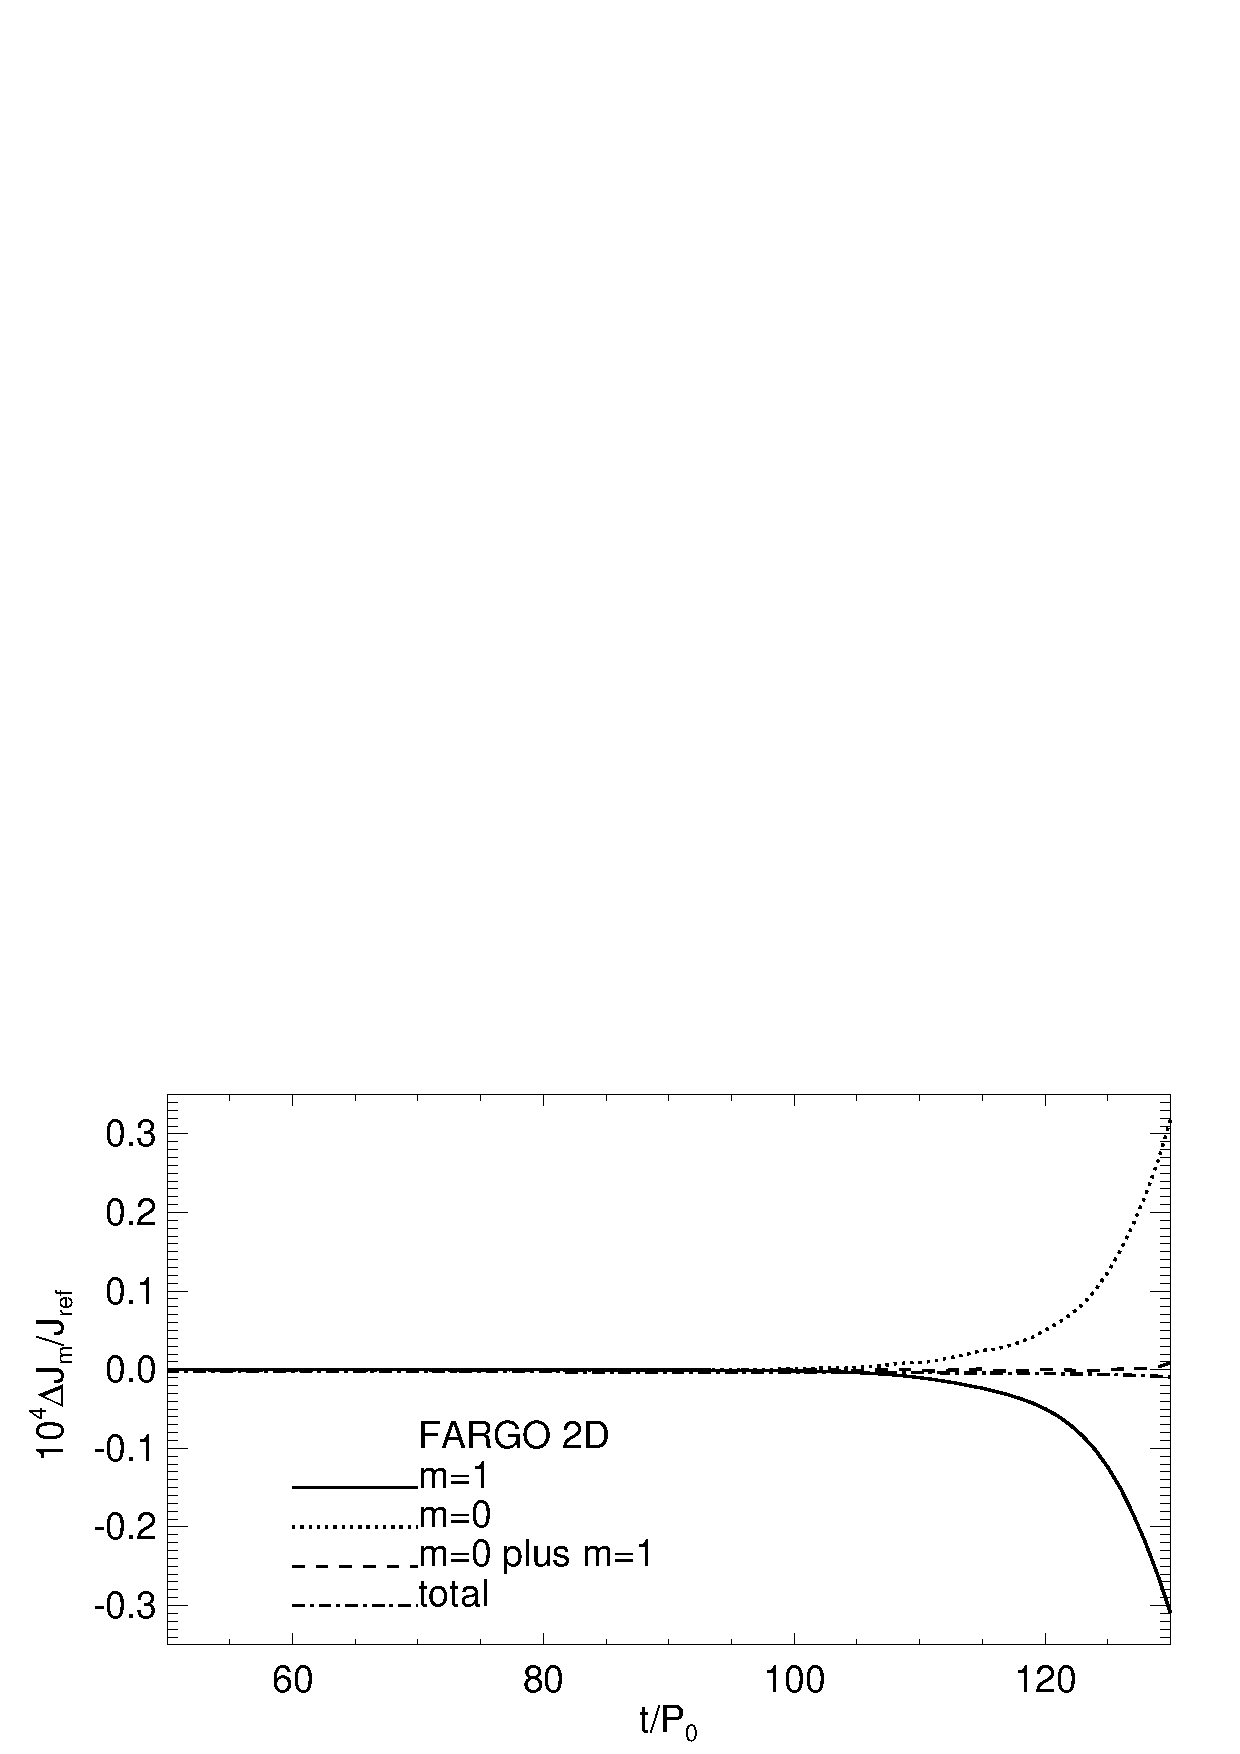
\includegraphics[width=\linewidth]{figures/nonaxi_evol_ang_fargo}
  \caption{Evolution of angular momentum components in the 
    FARGO simulation in Fig. \ref{fargo_modeamp}---\ref{fargo_2d}. The
    perturbation relative to $t=0$ in 2D is shown in units of the 
    initial total angular momentum $J_\mathrm{ref}$.\label{2d_angmom}} 
\end{figure}   

\subsection{Properties of the $m=1$ spiral and its growth}\label{fargo_m1}
In order to characterise the $m=1$ spiral that eventually
dominates, here we examine a simulation initialised with 
$M=1$ in Eq. \ref{randpert}. The one-armed spiral that emerges is more
coherent than the above simulation, which facilitates the analysis
below.   

Fig. \ref{2d_fargo_viz} shows a snapshot of the $m=1$ surface
density. By measuring the $m=1$ surface density amplitude and its
pattern speed, we obtain a co-rotation radius and growth rate 
\begin{align*}
  &R_c \simeq 4.4R_0,\\
  &\gamma\simeq 0.014\Omega_k(R_0) = 0.13\Omega_p. 
\end{align*}
This one-armed spiral can be considered as low frequency because its 
pattern speed $\Omega_p \simeq 0.1\Omega_k(R_0)\lesssim 0.3\Omega$ in
$R\in[R_{1},R_{2}]$ (where it has the largest amplitude). Thus, the spiral 
pattern appears nearly stationary. The growth rate $\gamma$ is also slow
relative to the local rotation, although the characteristic growth
time $\gamma^{-1} \simeq 10P_0$ is not very long.  
\begin{figure}
  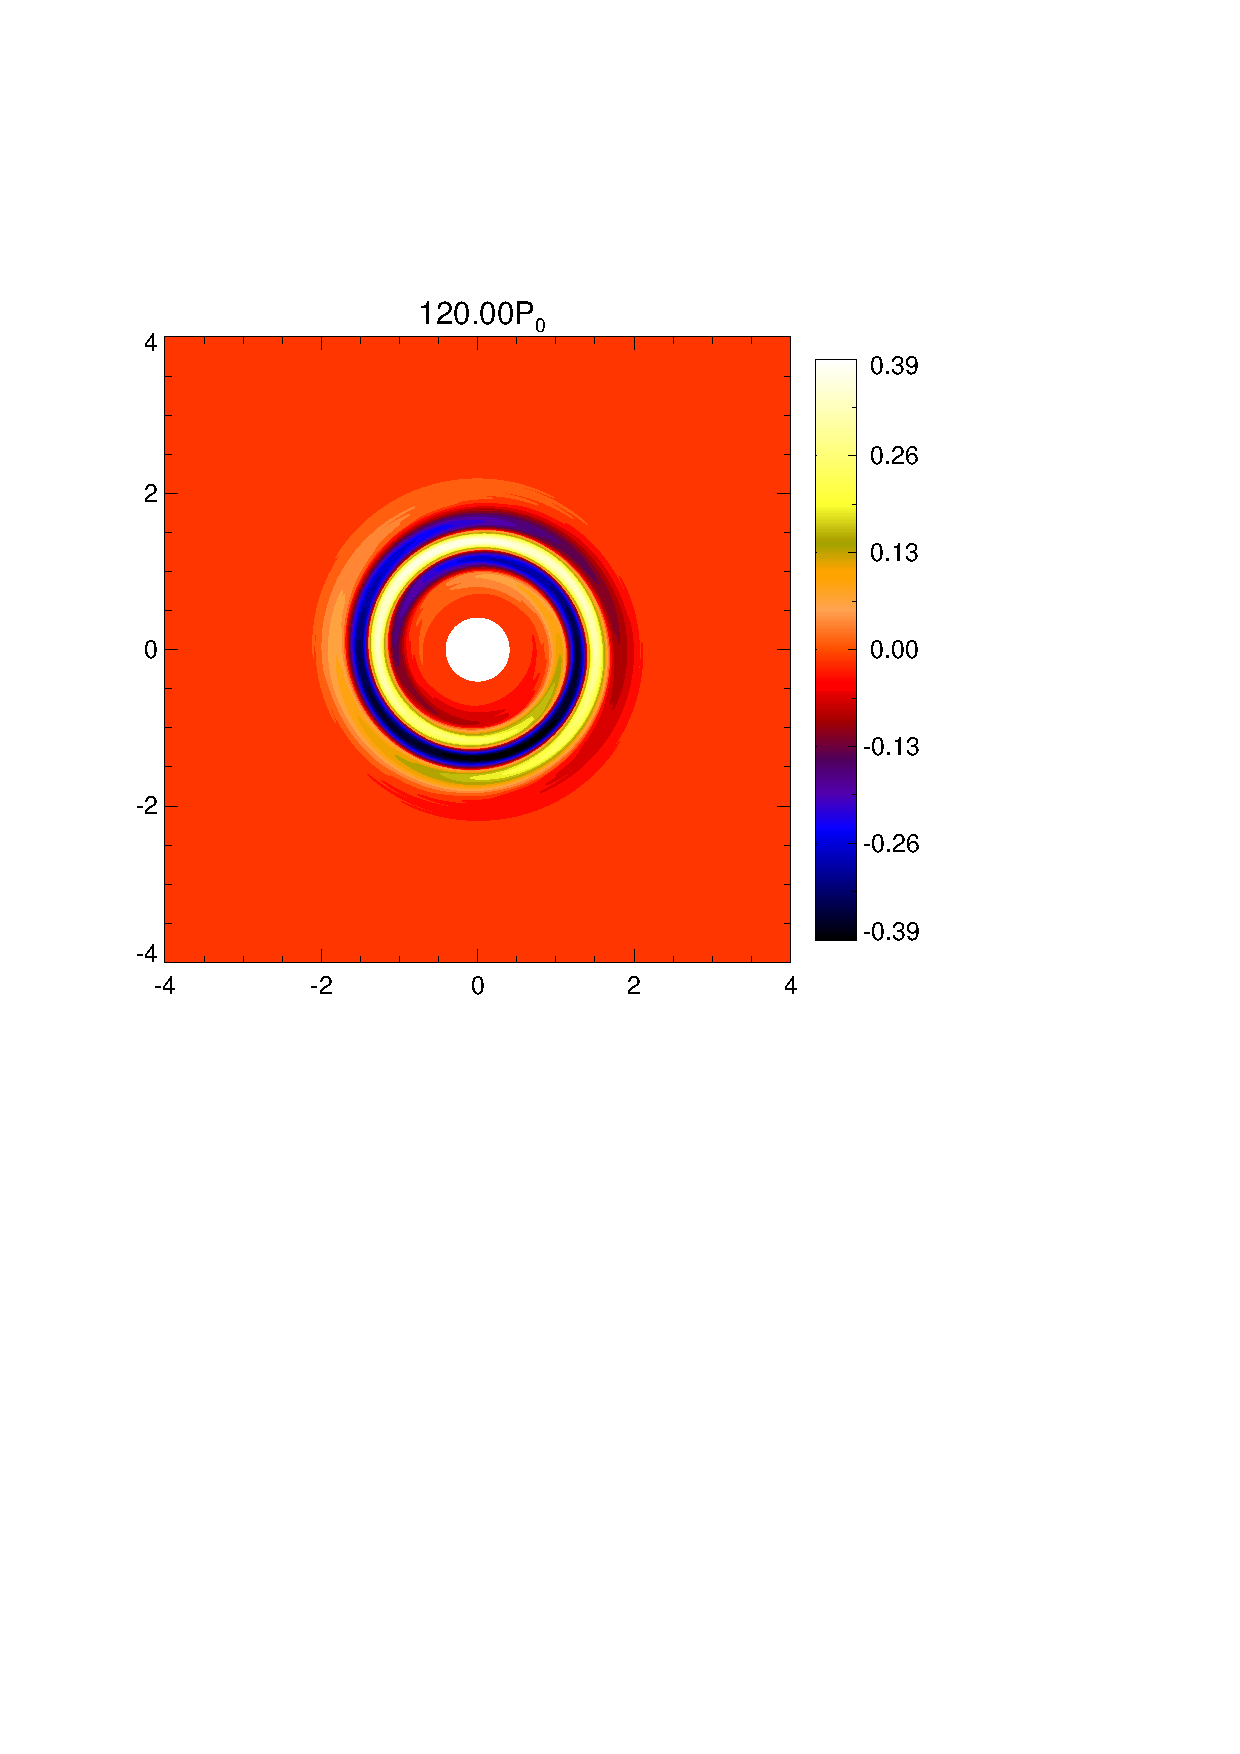
\includegraphics[width=\linewidth]{figures/polarxy2_dens120_fargo}
  \caption{Cartesian visualisation of the $m=1$ surface density
    structure in the FARGO simulation initialised with only $m=1$
    perturbations. 
    \label{2d_fargo_viz}} 
\end{figure}   

Next, we write $\Sigma_1 = 
|\Sigma_1|\exp{(\ii kR)}$, where $k$ is real, and assume the amplitude
$|\Sigma_1|$ varies slowly compared to the complex phase. This is the
main assumption in local theory. We calculate $k$ numerically and plot
its normalised value in Fig. \ref{fargo_wavenumber}. We find 
\begin{align*}
  kR \sim \frac{\pi G \Sigma}{c_s^2}R \sim \frac{1}{hQ}, 
\end{align*}
where we used $Q\sim c_s\Omega/\pi G \Sigma$ and $R\Omega/c_s\sim
h^{-1}$. Since $Q=O(1)$ and $h\ll 1$ imply $|kR|\gg 1$, we 
can apply results from local theory
self-consistently. Fig. \ref{2d_fargo_viz} shows the $m=1$ spiral is
trailing, which is consistent with $k>0$. 
 
%snapshot shows it's tightly wound
\begin{figure}
  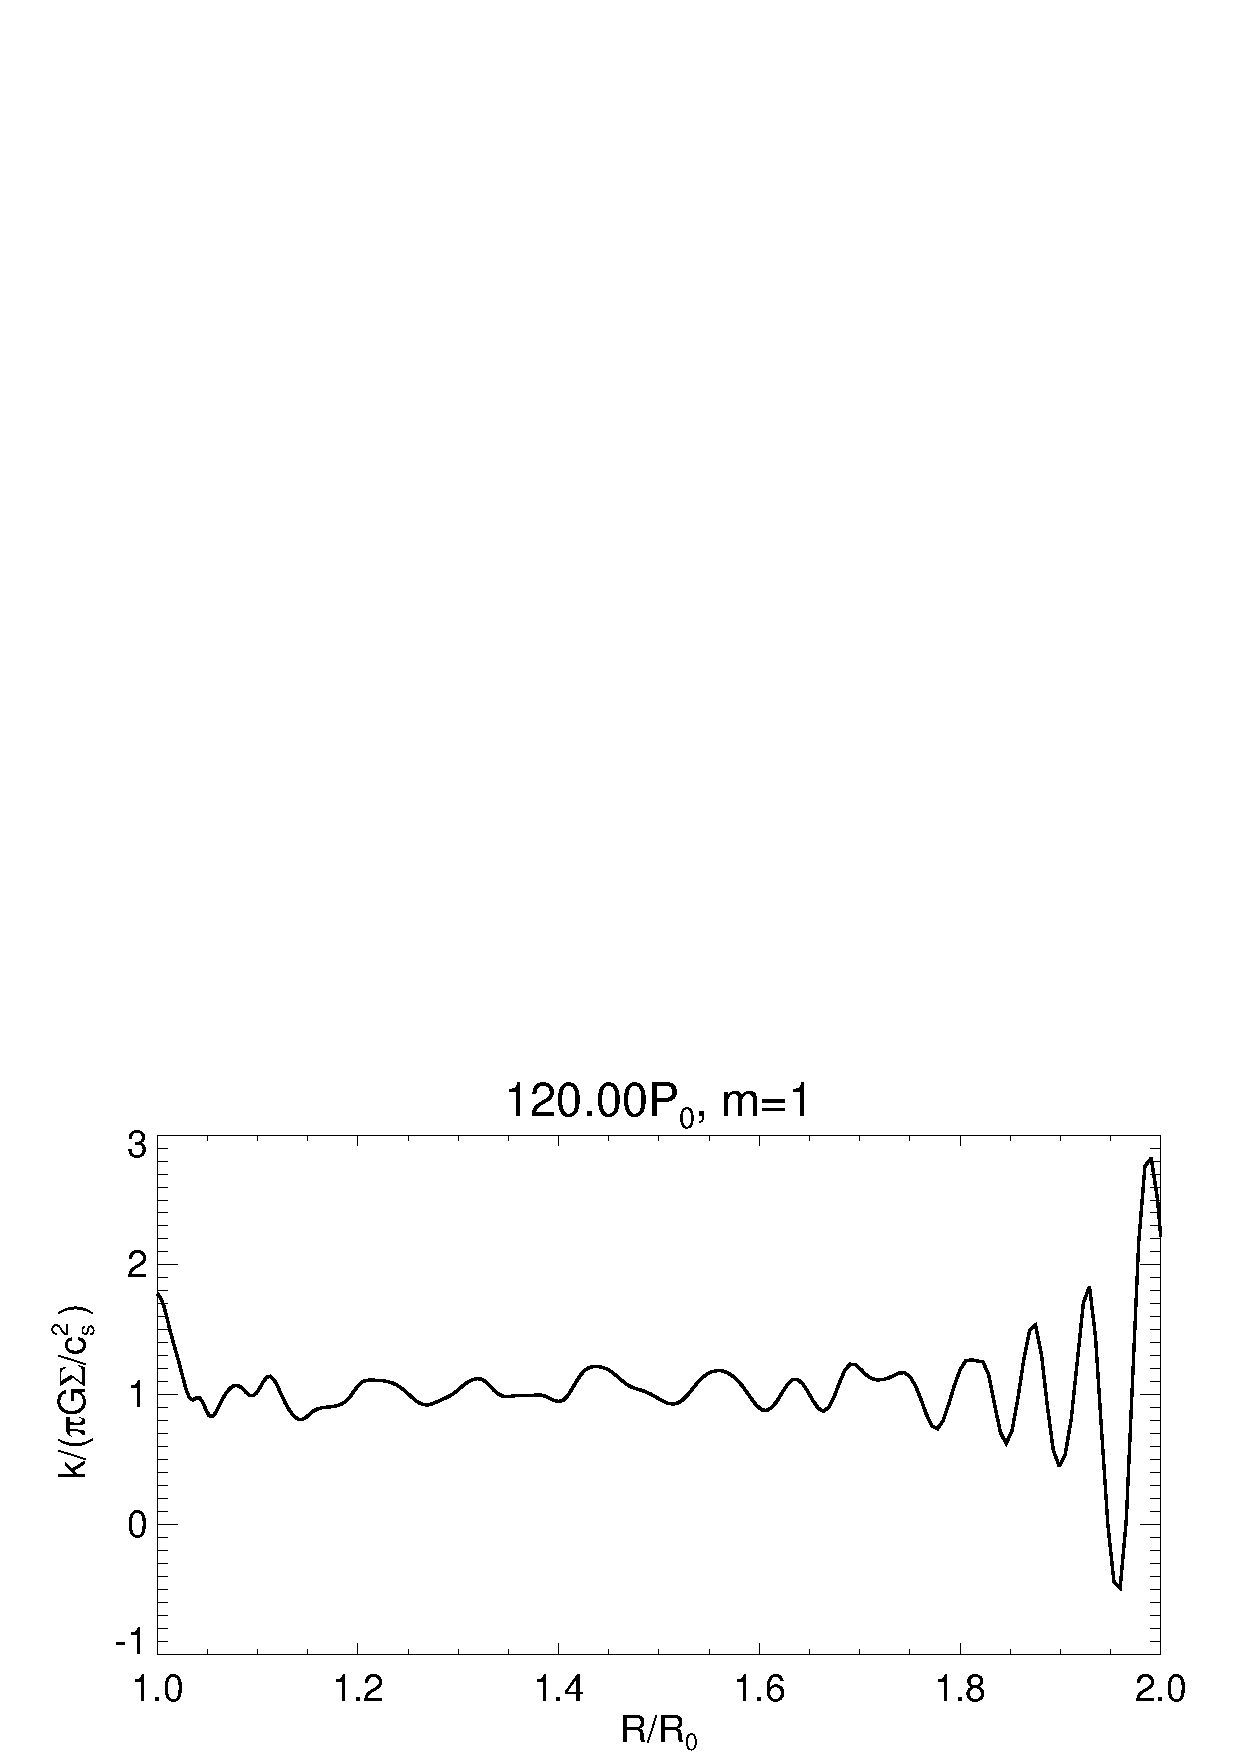
\includegraphics[width=\linewidth]{figures/m1_analysis_kr120_fargo}
  \caption{Normalised radial wavenumber of the $m=1$ spiral in 
    Fig. \ref{2d_fargo_viz}.\label{fargo_wavenumber}} 
\end{figure}   

%%%%%%%%%%%%%%%%%%%%%% 

Using the estimated value of $R_c$, we plot in
Fig. \ref{fargo_qbarrier} the quantity $\nu^2 - 1 + Q^{-2}$, which is
required to be positive in local theory for purely wave-like
solutions to the dispersion relation (Eq. \ref{dispersion}) when the
mode frequency is given. %Note that, with the above measured wavenumber $k$, 
%Eq. \ref{dispersion} requires $\nu^2 - 1 + Q^{-2}\sim0$ and the lower
%sign (long waves) to be taken. 
Fig. \ref{fargo_qbarrier} shows two $Q$-barriers located in
the inner disc, at $R_{Qb}=R_0$ and $R_{Qb}=1.6R_0$; the bounded region is indeed 
where the $m=1$ spiral develops. This suggests that the one-armed 
spiral is trapped. Note in this region, $\nu^2 - 1 + 
Q^{-2}\simeq 0.1\ll 1$, which is necessary for consistency with 
the measured wavenumber $k$ and Eq. \ref{wavenumber}.  
%Eq. \ref{dispersion} with the lower sign taken (i.e. long waves).  
There is one outer Lindblad resonance at $R_L\simeq
7.2R_0$. Thus, acoustic waves may be launched in $R\gtrsim 7.2R_0$ by
the spiral disturbance in the inner disc \citep{lin11b}. 
%implications: effect on dynamics in outer disc 

\begin{figure}
  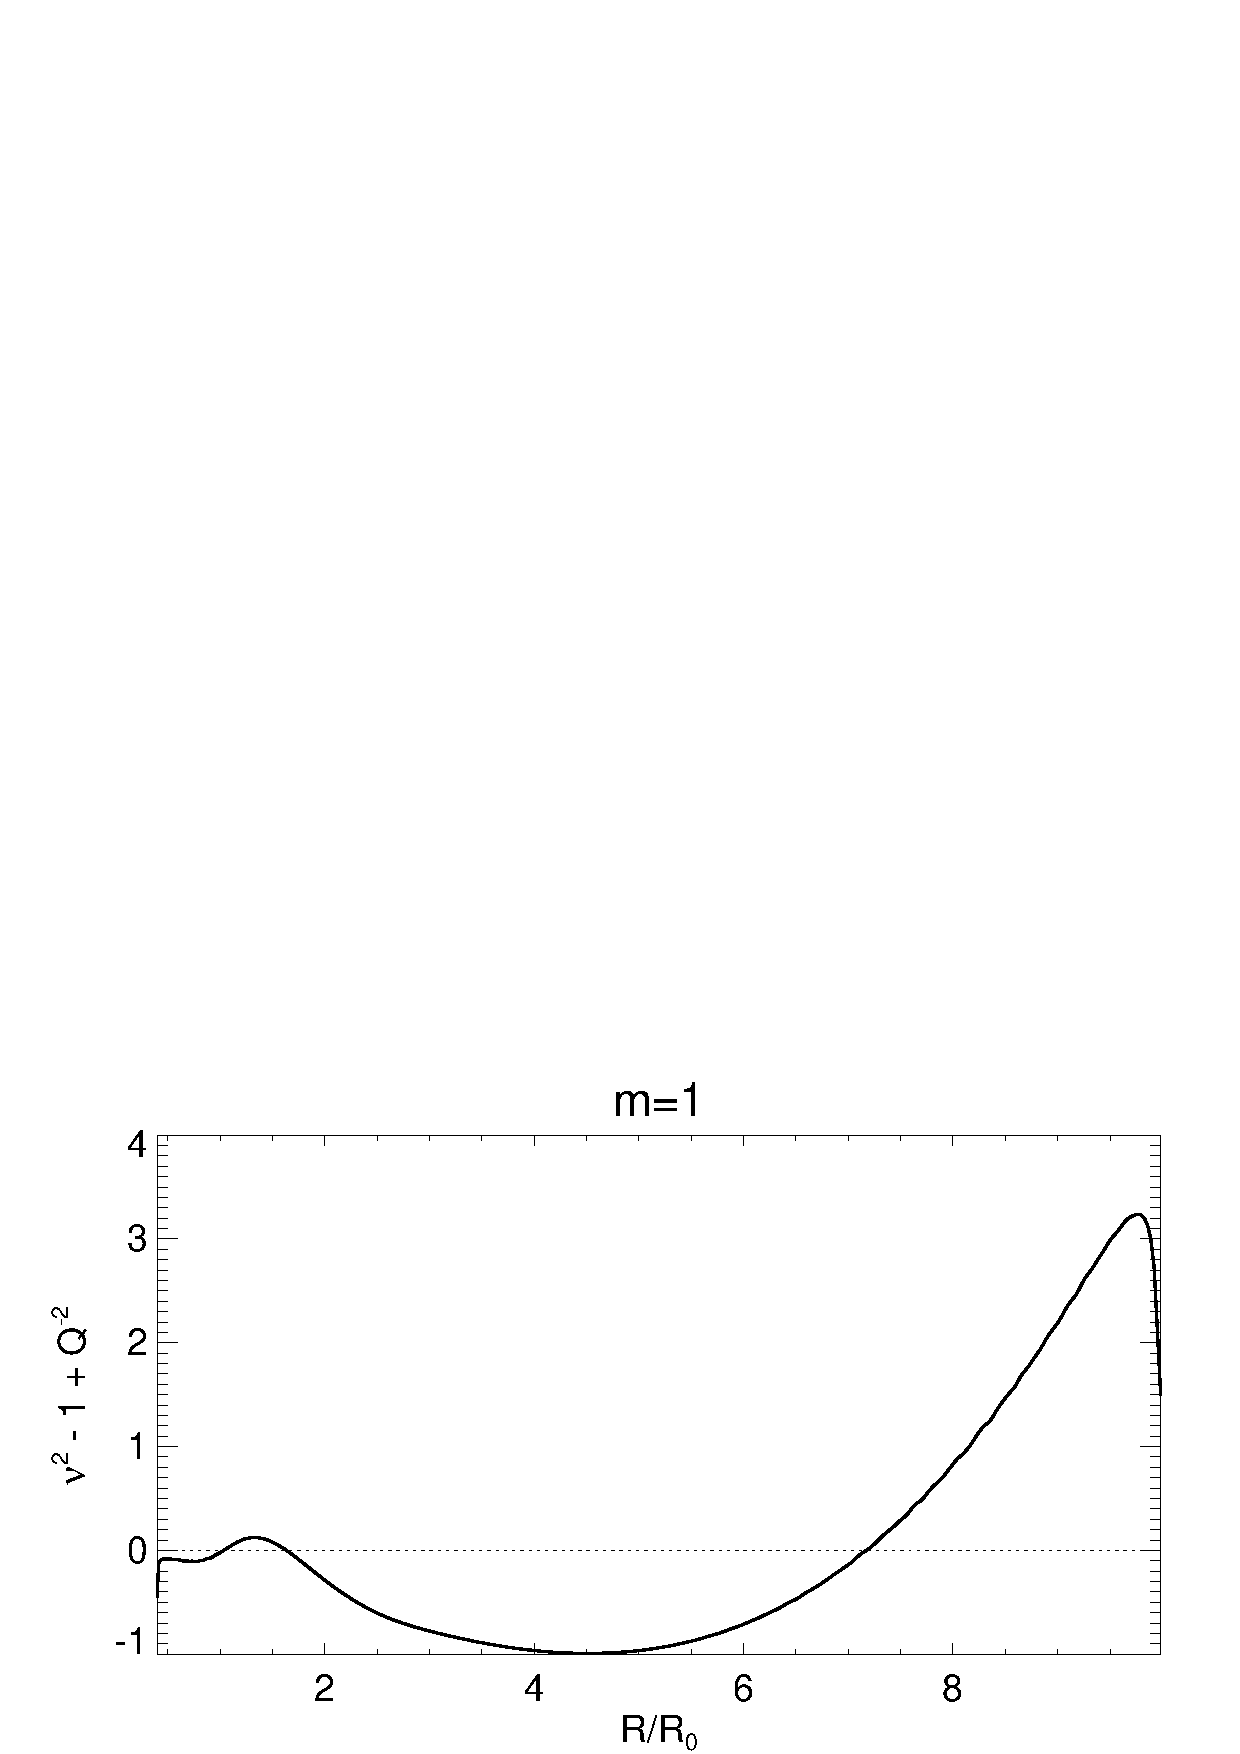
\includegraphics[width=\linewidth]{figures/m1_analysis_Qbar_fargo} 
  \caption{Dimensionless mode frequency $\nu$ for the $m=1$ spiral in
    Fig. \ref{2d_fargo_viz}. For a given real mode frequency, the
    dispersion relation for local density waves, Eq. \ref{dispersion},
    permits purely wave-like solutions in regions where $\nu^2 - 1 +
    Q^{-2}>0$.    
    \label{fargo_qbarrier}} 
\end{figure}

\subsubsection{Angular momentum exchange with the background disc}  
The wavenumber $k = \pi G\Sigma/c_s^2$ minimises the shifted frequency
$\sbar$ in the dispersion relation, Eq. \ref{dispersion}.  
Physically, then, it is not surprising to 
find perturbations of this wavenumber in a
self-gravitating disc where $Q\sim 1$. However, according the
local dispersion relation, $m=1$ perturbations are
formally stable for real $k$ and $Q>1$.   

%most of the perturbation is inside co-rotation 
%so resonant interaction unlikely for instability 

In order to track down the origin for the (slow) growth of the
$m=1$ spiral, we invoke angular momentum conservation for linear
perturbations, Eq. \ref{lin_ang_mom_cons}. Assuming fluxes are
negligible at the disc boundaries, we can integrate
Eq. \ref{lin_ang_mom_cons} to give
\begin{align}\label{baroclinic_torque_int}
  \frac{d}{dt}\underbrace{\int_{R_\mathrm{min}}^{R_\mathrm{max}}\jlin
    2\pi R dR}_{\jlintot} 
  =\int_{R\mathrm{min}}^{R\mathrm{max}}T_\mathrm{BG} 2\pi R dR, 
\end{align}
where we recall $T_\mathrm{BG}$ is the torque density due to the imposed
sound-speed profile (Eq. \ref{baroclinic_torque}). We explicitly 
compute both sides of Eq. \ref{baroclinic_torque_int} using
simulation data, and compare them in Fig. \ref{fargo_angmom_ex}. There
is a good match between the two torques, especially at early times
$t\lesssim110P_0$. The average discrepancy is $\simeq 5\%$. 
The match is less good later on, when the spiral
amplitude is no longer small ($\Delta\Sigma_1\sim 0.2$ at $t=110P_0$
and $\Delta\Sigma_1\sim 0.4$ by $t=120P_0$) and linear theory becomes
less applicable. Fig. \ref{fargo_angmom_ex} confirms that the $m=1$ spiral
wave experiences a negative torque that further reduces its angular
momentum. This is consistent with angular momentum component
measurements (Fig. \ref {2d_angmom}).  

% similar results if only intergrating between R_1 and R_2
%wave losses at boundaries 

\begin{figure}
  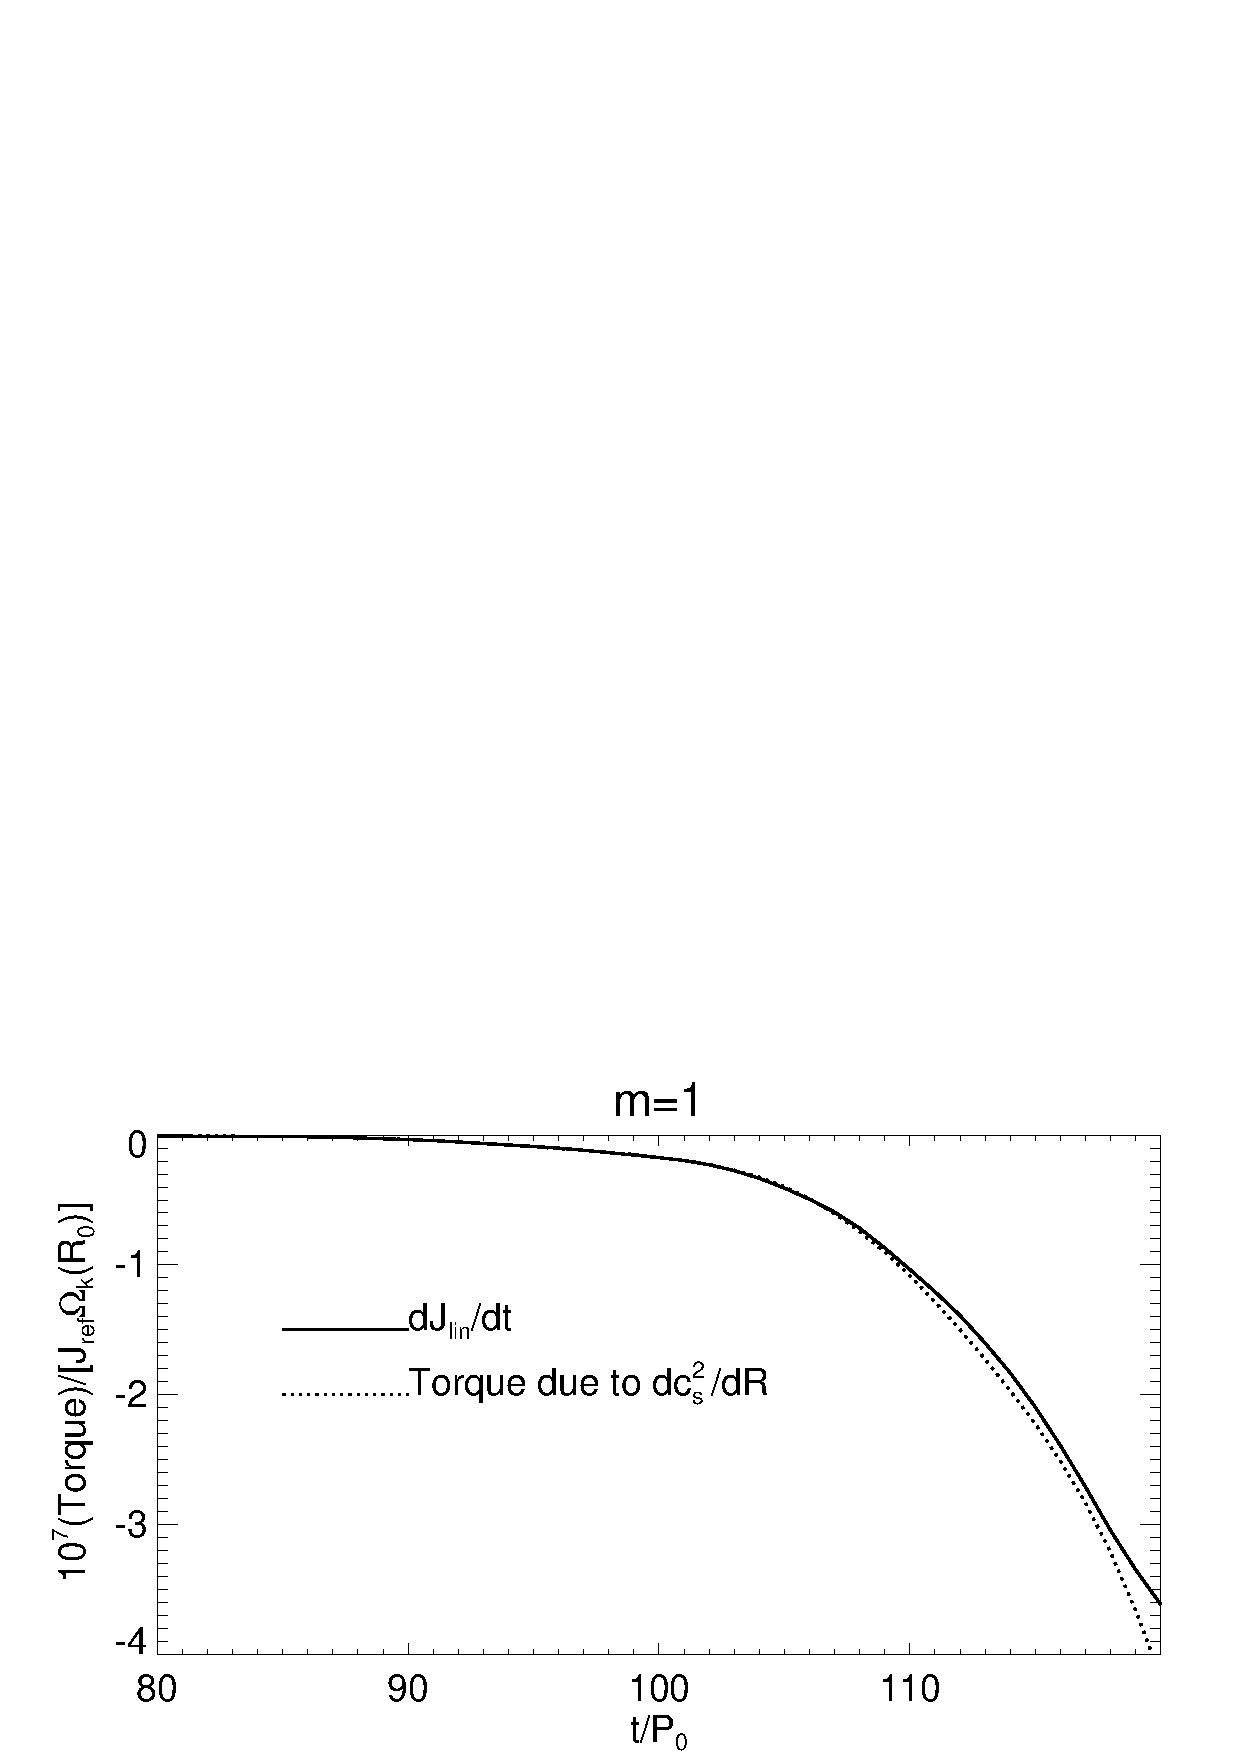
\includegraphics[width=\linewidth]{figures/m1_analysis_ang_fargo} 
  \caption{Rate of change of the $m=1$ wave angular momentum as defined by
    Eq. \ref{baroclinic_torque_int} (solid) compared to the torque
    exerted on the wave associated with the background temperature
    gradient (dotted). 
    \label{fargo_angmom_ex}} 
\end{figure}

%ang mom decreases slightly more rapidly than torque exchange provides
%- probably non-linear effects/shocks 

\subsection{Dependence on the imposed temperature profile}
The simulations above suggest the growth of the $m=1$ spiral mode
can be attributed to the background torque applied on linear perturbations
as a result of an imposed temperature gradient, as discussed in
\S\ref{global_cons}. According to Eq. \ref{baroclinic_torque}, this
torque is proportional to $q$, the power-law index used to set the
sound-speed profile (Eq. \ref{sound-speed}) in our simulations. 
We confirm this through a series of simulations with $q\in[0,1]$, 
initialised with $m=1$ perturbations. However, to keep the Toomre $Q$
profiles similar, we adjust the surface density power-law index such
that $s = (3+q)/2$.  

Fig. \ref{fargo_varq} compares the $m=1$ spiral amplitudes as a
function of $q$. We indeed observe slower growth with decreasing
$q$. Although the figure indicates growth for the strictly isothermal
disc ($q=0$), we did not observe a coherent one-armed spiral upon
inspection of the $m=1$ surface density field. The growth in this case
may be associated with high-$m$ modes, which dominated the
simulation.   

% difficult to measure  
% show result of isothermal calc?

\begin{figure}
  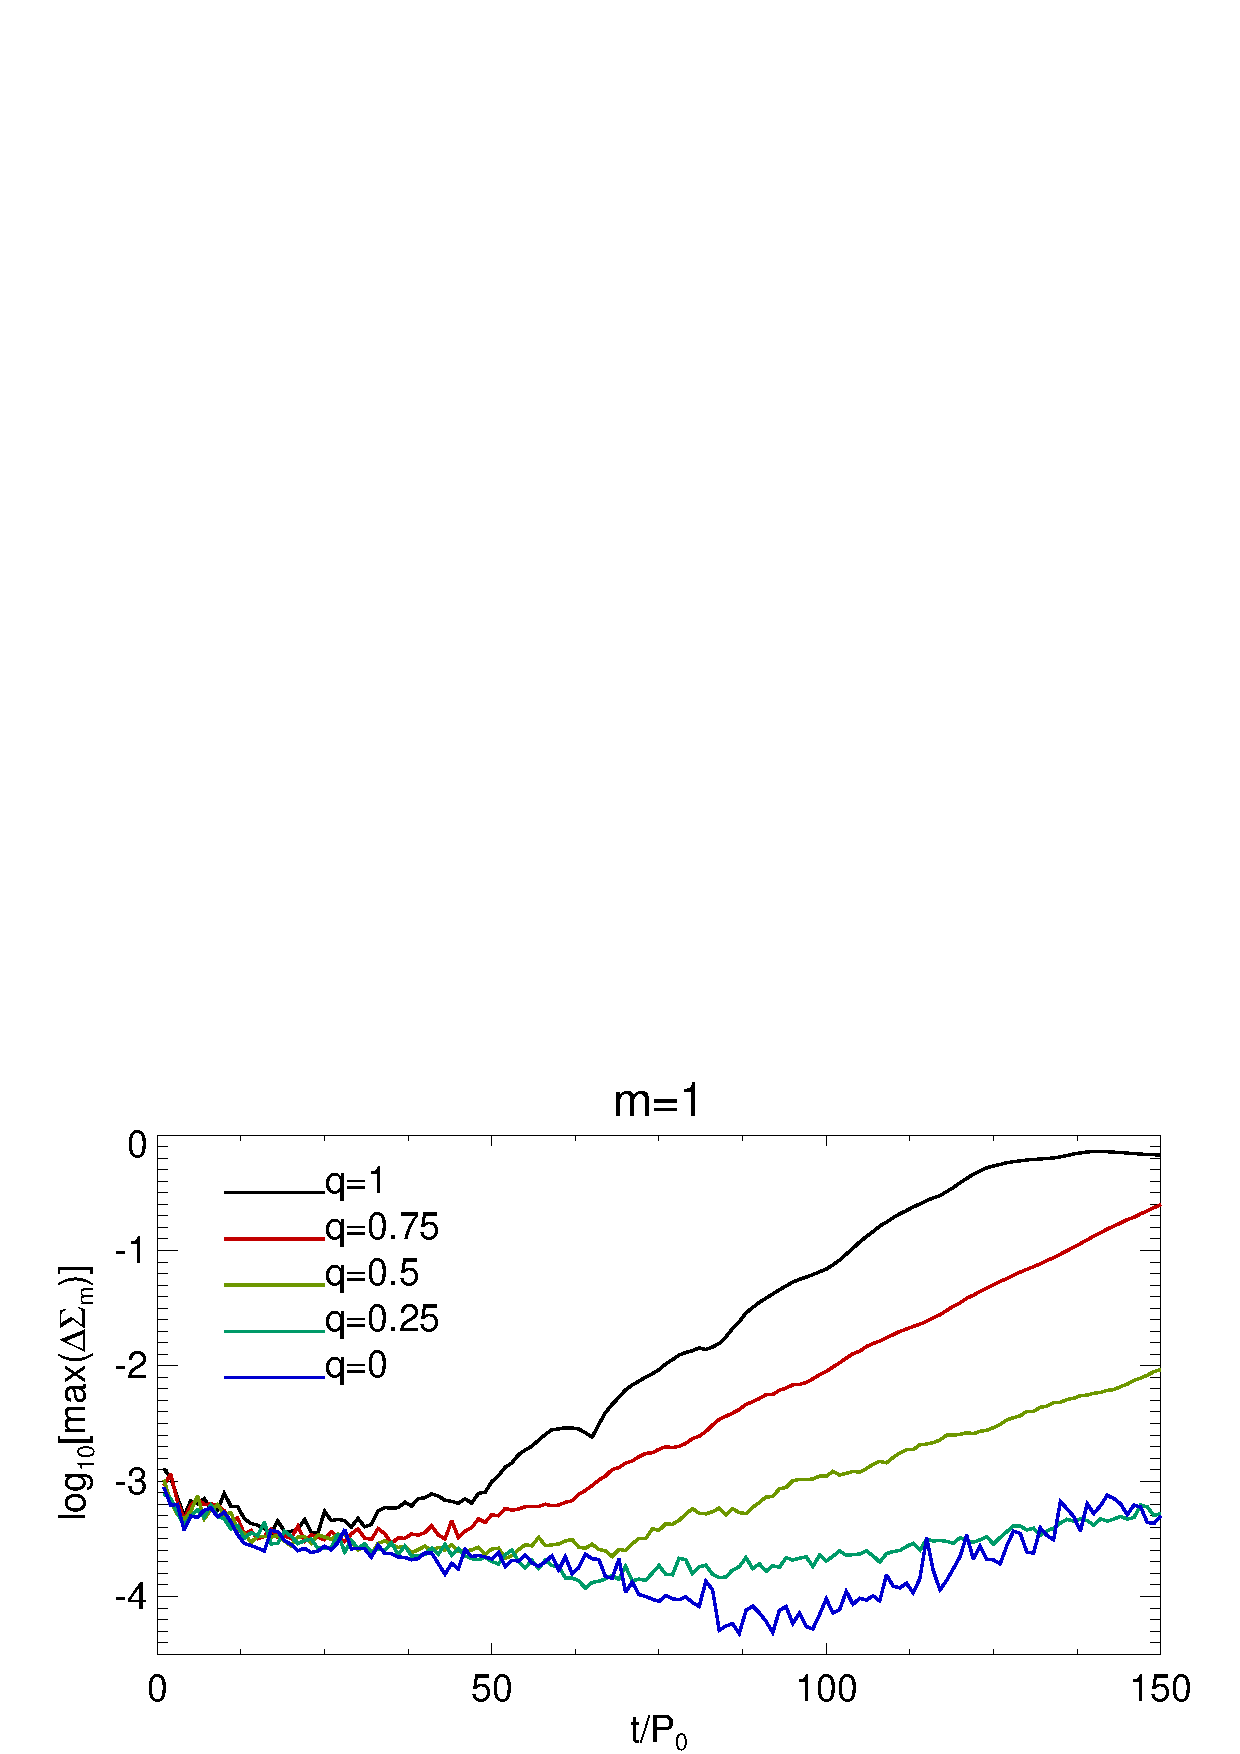
\includegraphics[width=\linewidth]{figures/m1_analysis_plot_fargo_varq}   
  \caption{Evolution of the $m=1$ spiral amplitude as a function of
    the imposed sound-speed gradient $q$. The maximum value of the
    $m=1$ surface density in $R\in[R_1,R_2]$ is shown. 
    \label{fargo_varq}} 
\end{figure}
We plot growth rates of the $m=1$ spiral as a function of $q$ in 
Fig. \ref{fargo_varq_growth}. The correlation can be fitted with a 
linear relation
\begin{align*}
  \gamma \simeq \left[0.015 q - 7.9\times10^{-4}\right] \Omega_k(R_0). 
\end{align*}
% difficult to measure very small growth rates
This shows that the temperature gradient is responsible for the
development of the one-armed spirals observed in our simulations.  

\begin{figure}
  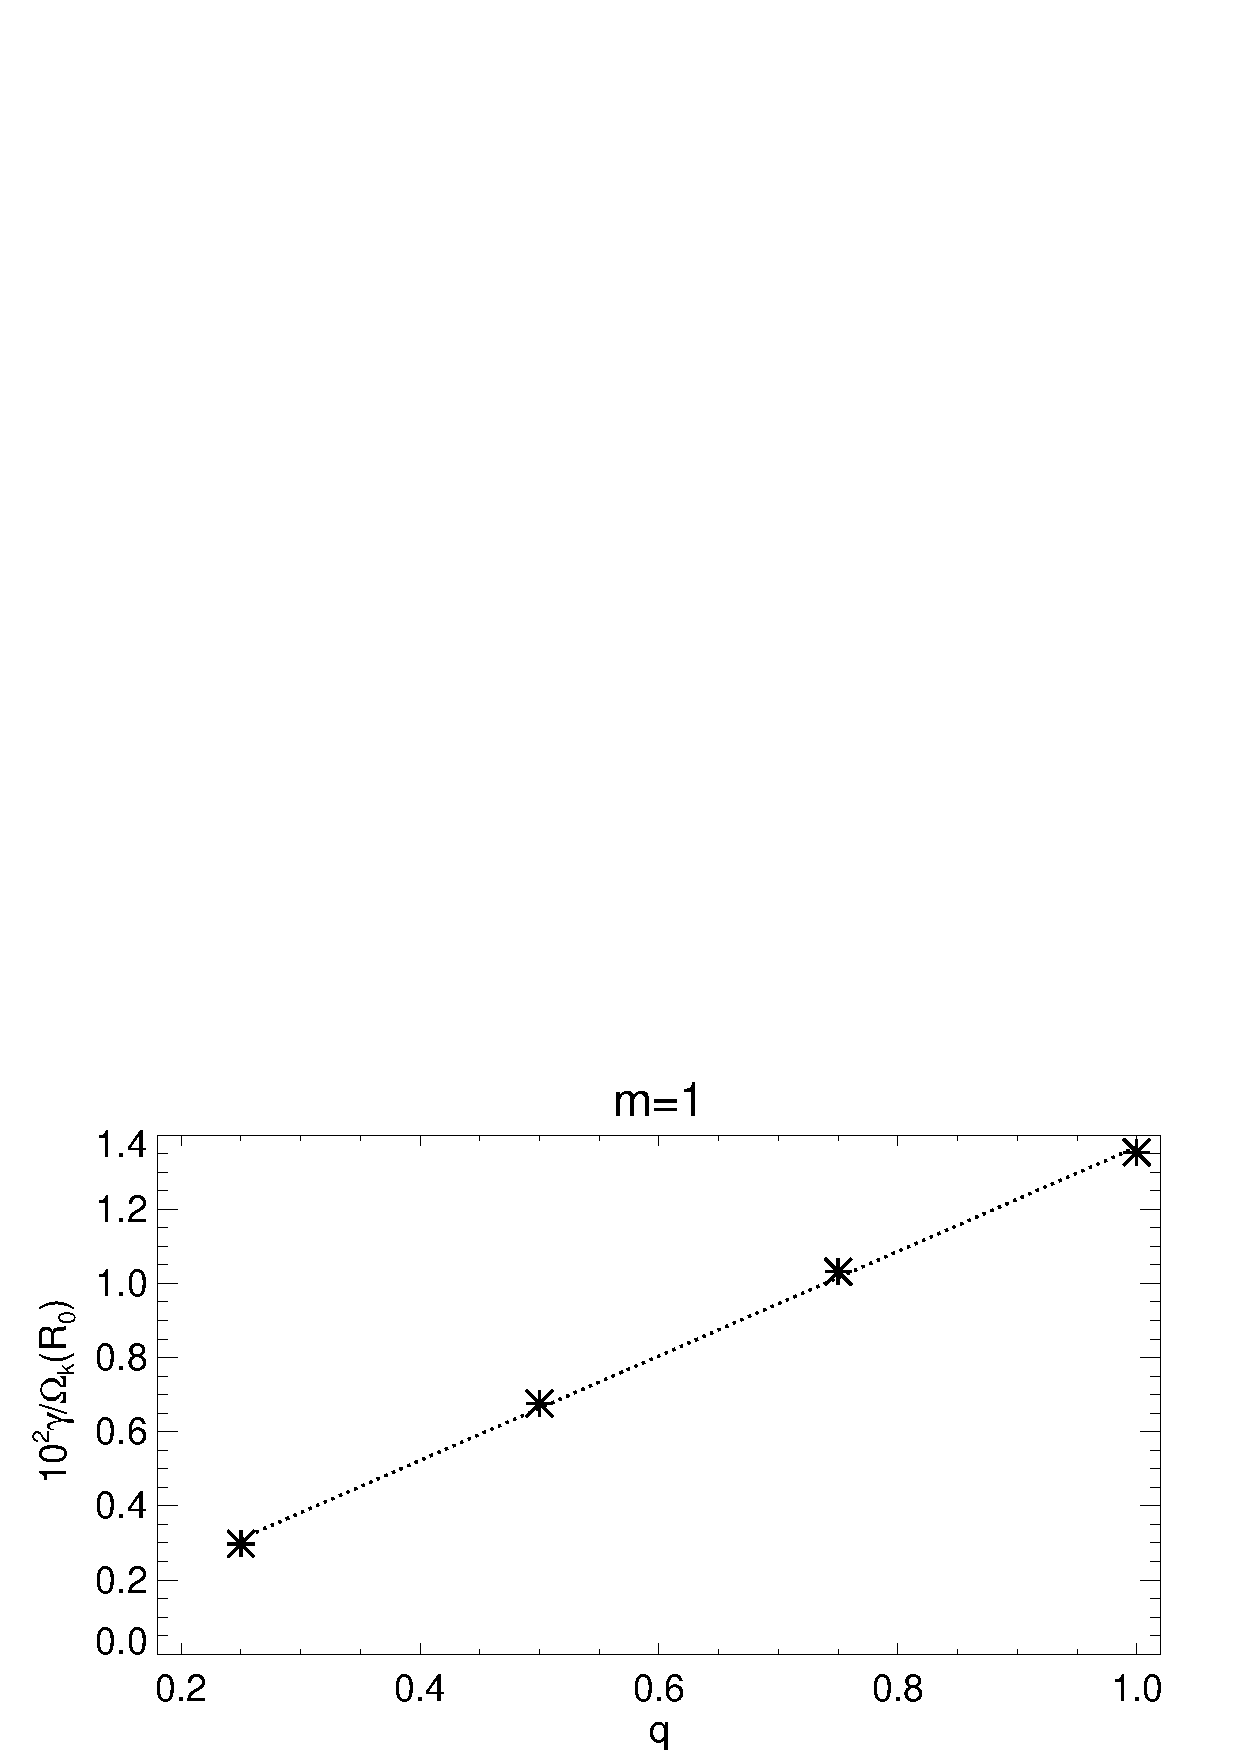
\includegraphics[width=\linewidth]{figures/m1_analysis_plot_ratemax_fargo_varq}    
  \caption{Growth rates of the $m=1$ spiral mode as a function of the
    imposed sound-speed gradient $q$ (asterisks). A linear fit is also 
    plotted (dotted line). 
    \label{fargo_varq_growth}} 
\end{figure}
%maybe extend the low q simulations to get better rates?

We also performed a series of simulations with variable aspect-ratio 
$h\in[0.03,0.07]$ but fixed $q=1$. This affects the magnitude of the temperature
gradient since $c_s \propto h$. However, with other parameters equal
to that in the fiducial simulation,  varying $h$ also changes the disc
mass. For $h\in[0.03,0.07]$ the total disc mass ranges from
$M_d=0.052M_*$ to $M_d=0.12M_*$ and the 
mass within $R\in[R_1,R_2]$  ranges from $0.033M_*$ to $0.062M_*$. 
% similar Q profiles

Fig. \ref{fargo_varh_growth} shows the growth rates of the $m=1$
spiral in $R\in[R_1,R_2]$ as a function of $h$. Growth rates increases
with $h$, roughly as  
\begin{align*}
  \gamma \simeq \left[0.10h + 8.3\times10^{-3}\right]\Omega_k(R_0).  
\end{align*}
However, a linear fit is less good than for variable $q$ cases above. This
may be due to the change in the total disc mass when $h$ changes. We
find no qualitative difference between the spiral pattern that
emerges. 

\begin{figure}
  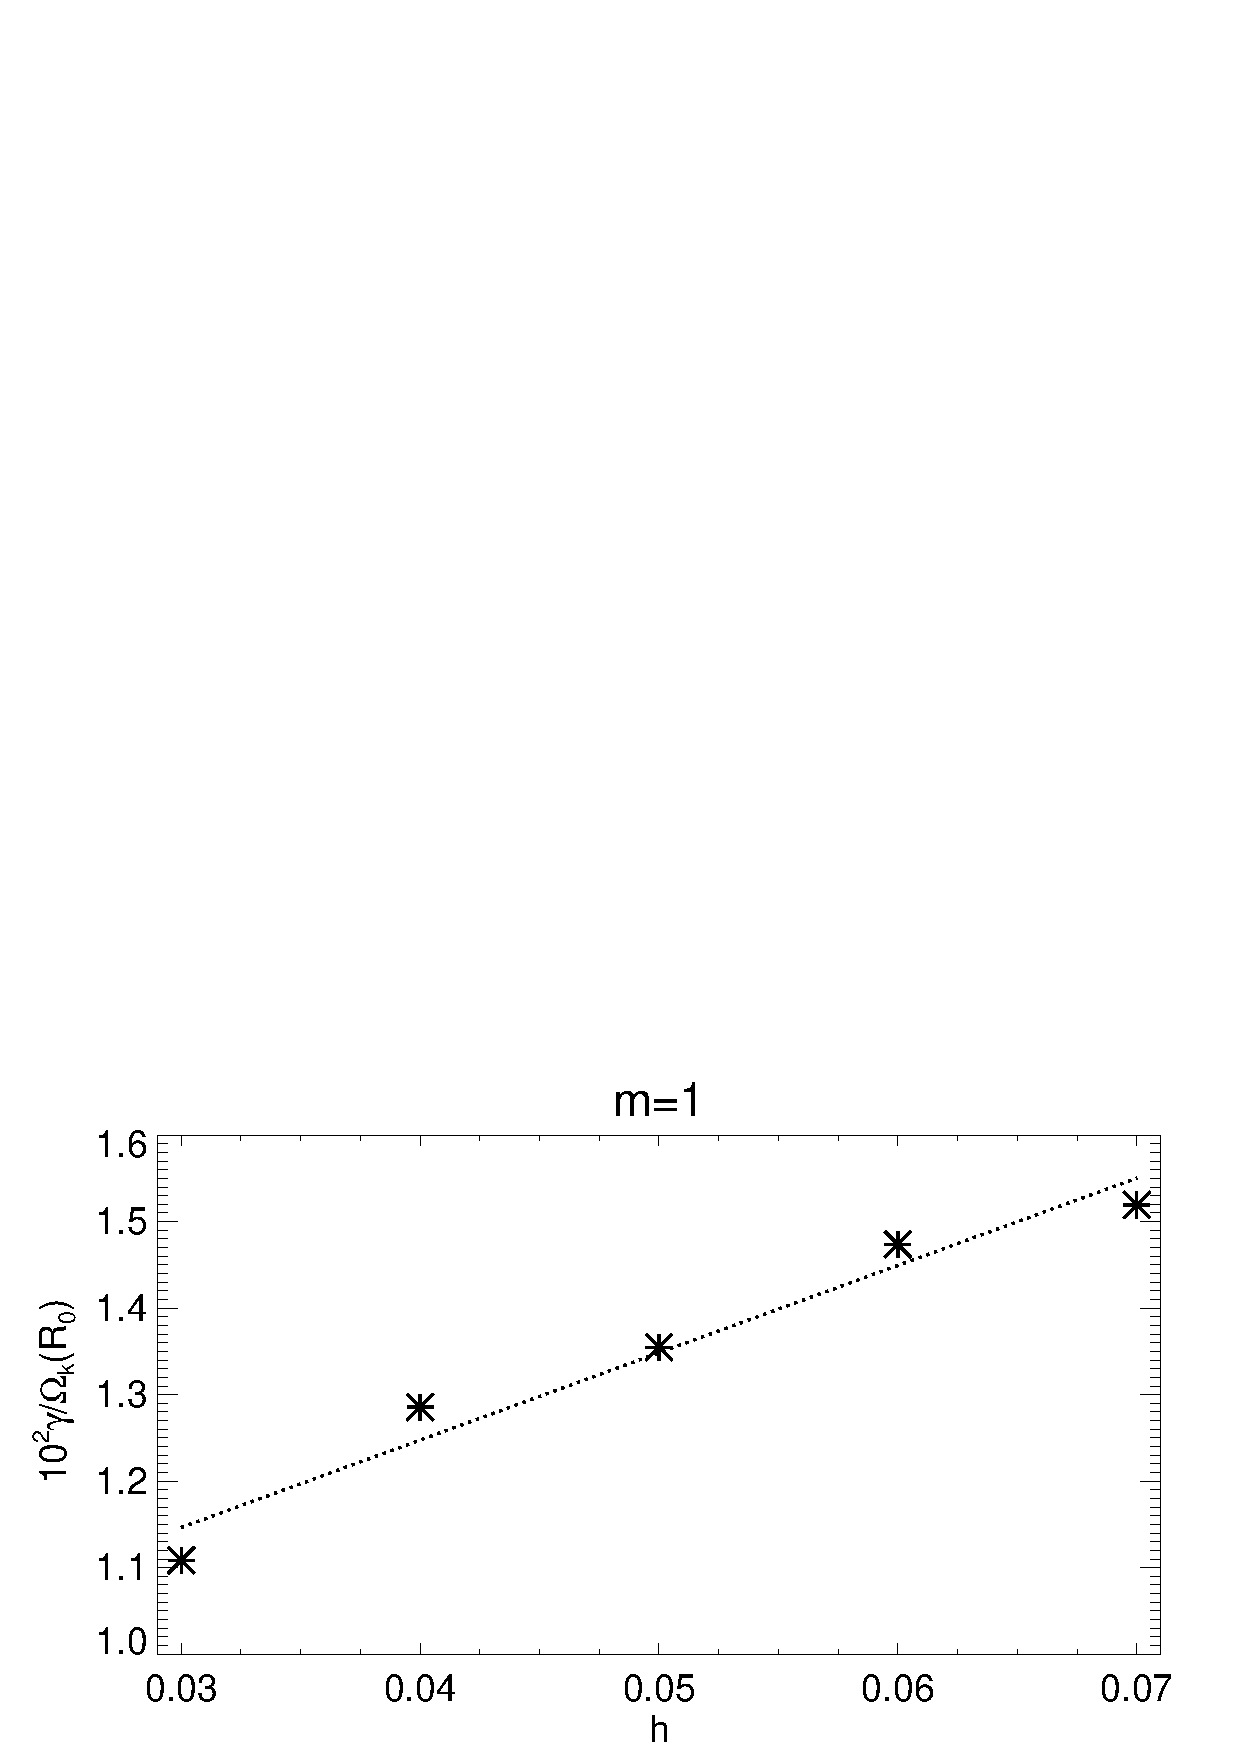
\includegraphics[width=\linewidth]{figures/m1_analysis_plot_ratemax_fargo_varh}    
  \caption{Growth rates of the $m=1$ spiral mode as a function of the
    disc aspect-ratio $h$ (asterisks). A linear fit is also
    plotted (dotted line). 
    \label{fargo_varh_growth}} 
\end{figure}
